\subsection*{1.3 Linear Equation in Two Varibles}

\vspace{0.5em}

\setcounter{questionnum}{0}

\noindent\markforreview

\vspace{1em}

The table gives the coordinates of two points on a line in the $xy$-plane. The $y$-intercept of the line is $(k - 5, b)$, where $k$ and $b$ are constants. What is the value of $b$?

\[
\begin{array}{c|c}
x & y \\
\hline
k & 13 \\
k + 7 & -15 \\
\end{array}
\]

\vspace{0.75em}


\vspace{2em}

\noindent\markforreview

\vspace{1em}

The graph of the equation $ax + ky = 6$ is a line in the $xy$-plane, where $a$ and $k$ are constants. If the line contains the points $(-2, -6)$ and $(0, -3)$, what is the value of $k$?

\vspace{0.75em}

\choicebox{A}{$-2$}
\choicebox{B}{$-1$}
\choicebox{C}{$2$}
\choicebox{D}{$3$}

\newpage
\noindent\markforreview

\vspace{1em}

For line $h$, the table shows three values of $x$ and their corresponding values of $y$. Line $k$ is the result of translating line $h$ down 5 units in the $xy$-plane. What is the $x$-intercept of line $k$?

\[
\begin{array}{c|c}
x & y \\
\hline
18 & 130 \\
23 & 160 \\
26 & 178 \\
\end{array}
\]

\vspace{0.75em}

\choicebox{A}{$\left( -\frac{26}{3}, 0 \right)$}
\choicebox{B}{$\left( -\frac{9}{2}, 0 \right)$}
\choicebox{C}{$\left( -\frac{11}{3}, 0 \right)$}
\choicebox{D}{$\left( -\frac{17}{6}, 0 \right)$}

\vspace{2em}

\noindent\markforreview

\vspace{1em}

A certain apprentice has enrolled in 85 hours of training courses. The equation $10x + 15y = 85$ represents this situation, where $x$ is the number of on-site training courses and $y$ is the number of online training courses this apprentice has enrolled in. How many more hours does each online training course take than each on-site training course?

\newpage
\noindent\markforreview

\vspace{1em}

Line $p$ is defined by $4y + 8x = 6$. Line $r$ is perpendicular to line $p$ in the $xy$-plane. What is the slope of line $r$?


\vspace{15em}

\noindent\markforreview

\vspace{1em}

In the $xy$-plane, line $k$ intersects the $y$-axis at the point $(0, -6)$ and passes through the point $(2, 2)$. If the point $(20, w)$ lies on line $k$, what is the value of $w$?


\vspace{15em}

\noindent\markforreview

\vspace{1em}

In the $xy$-plane, line $\ell$ passes through the point $(0, 0)$ and is parallel to the line represented by the equation $y = 8x + 2$. If line $\ell$ also passes through the point $(3, d)$, what is the value of $d$?

\vspace{2em}

\newpage
\noindent\markforreview

\vspace{1em}
\begin{center}
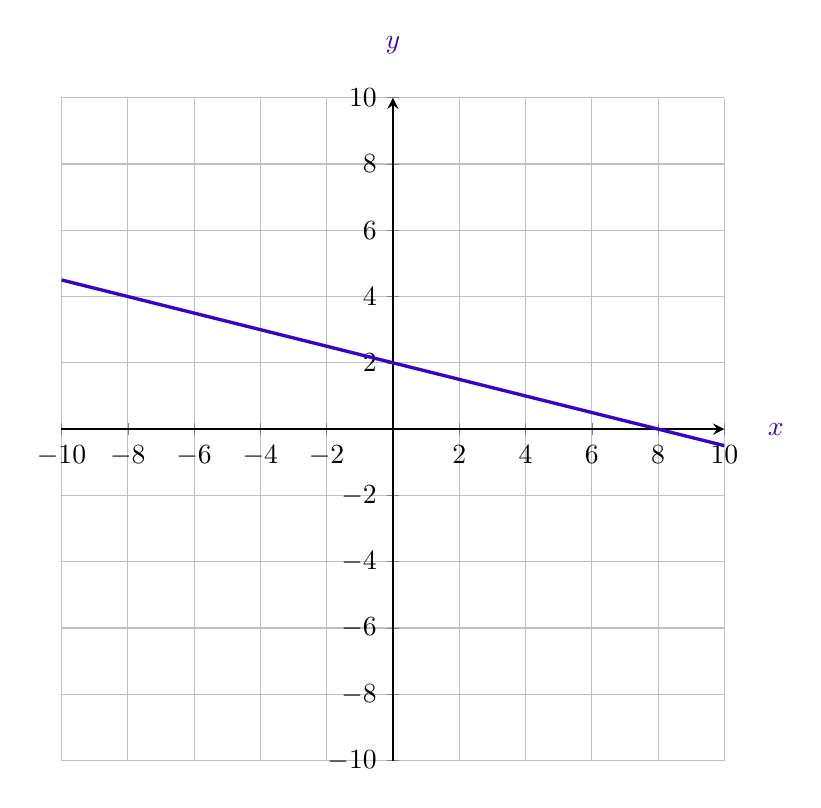
\begin{tikzpicture}
  \begin{axis}[
    axis lines=middle,
    % 紫蓝色刻度线
    xmin=-10, xmax=10,
    ymin=-10, ymax=10,
    xtick={-10,-8,...,10},
    ytick={-10,-8,...,10},
    grid=both,
    width=10cm,
    height=10cm,
    enlargelimits=false,
    xlabel={$x$}, ylabel={$y$},
    every axis x label/.style={
      at={(ticklabel* cs:1.05)}, anchor=west, color=purple!30!blue, font=\bfseries
    },
    every axis y label/.style={
      at={(ticklabel* cs:1.05)}, anchor=south, color=purple!30!blue, font=\bfseries
    },
    domain=-10:10,
    samples=2,
    thick
  ]
    \addplot [purple!30!blue, very thick] {-0.25*x + 2};
  \end{axis}
\end{tikzpicture}
\end{center}
\vspace{0.75em}

The graph of \( y = f(x) + 14 \) is shown. Which equation defines function \( f \)?

\vspace{0.75em}

\choicebox{A}{$f(x) = -\frac{1}{4}x - 12$}
\choicebox{B}{$f(x) = -\frac{1}{4}x + 16$}
\choicebox{C}{$f(x) = -\frac{1}{4}x + 2$}
\choicebox{D}{$f(x) = -\frac{1}{4}x - 14$}


\newpage


\noindent\markforreview

\vspace{1em}

Keenan made \textbf{32} cups of vegetable broth. Keenan then filled \( x \) small jars and \( y \) large jars with all the vegetable broth he made. The equation \( 3x + 5y = 32 \) represents this situation. Which is the best interpretation of \( 5y \) in this context?

\vspace{0.75em}

\choicebox{A}{The number of large jars Keenan filled}
\choicebox{B}{The number of small jars Keenan filled}
\choicebox{C}{The total number of cups of vegetable broth in the large jars}
\choicebox{D}{The total number of cups of vegetable broth in the small jars}

\newpage

\noindent\markforreview

\vspace{1em}

\[ax+by=b\]

In the equation above, \( a \) and \( b \) are constants and \( 0 < a < b \). Which of the following could represent the graph of the equation in the \( xy \)-plane?

\textbf{For each length of the square, it counts 0.5}




\choicebox{A}{%
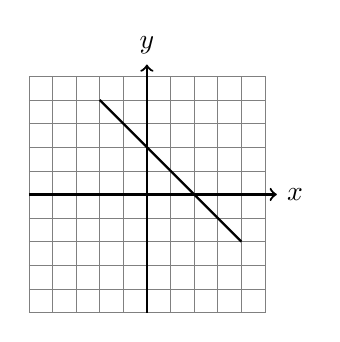
\begin{tikzpicture}[scale=0.3]
  \draw[step=1cm,gray,very thin] (-5,-5) grid (5,5);
  \draw[->,thick] (-5,0) -- (5.5,0) node[right] {$x$};
  \draw[->,thick] (0,-5) -- (0,5.5) node[above] {$y$};
  \draw[thick] (-2,4) -- (4,-2);
\end{tikzpicture}}


\choicebox{B}{%
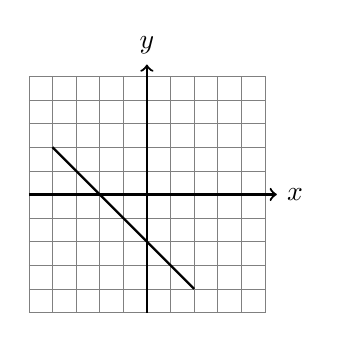
\begin{tikzpicture}[scale=0.3]
  \draw[step=1cm,gray,very thin] (-5,-5) grid (5,5);
  \draw[->,thick] (-5,0) -- (5.5,0) node[right] {$x$};
  \draw[->,thick] (0,-5) -- (0,5.5) node[above] {$y$};
  \draw[thick] (-4,2) -- (2,-4);
\end{tikzpicture}}

\choicebox{C}{%
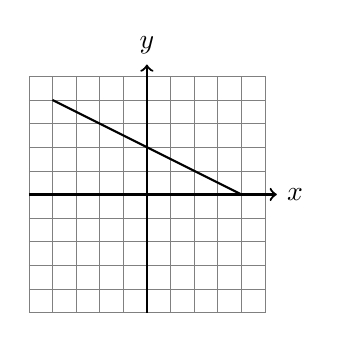
\begin{tikzpicture}[scale=0.3]
  \draw[step=1cm,gray,very thin] (-5,-5) grid (5,5);
  \draw[->,thick] (-5,0) -- (5.5,0) node[right] {$x$};
  \draw[->,thick] (0,-5) -- (0,5.5) node[above] {$y$};
  \draw[thick] (4,0) -- (-4,4);
\end{tikzpicture}}

\choicebox{D}{%
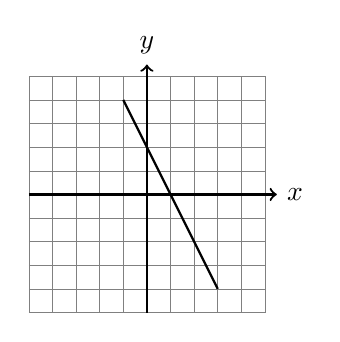
\begin{tikzpicture}[scale=0.3]
  \draw[step=1cm,gray,very thin] (-5,-5) grid (5,5);
  \draw[->,thick] (-5,0) -- (5.5,0) node[right] {$x$};
  \draw[->,thick] (0,-5) -- (0,5.5) node[above] {$y$};
  \draw[thick] (3,-4) -- (-1,4);
\end{tikzpicture}}


\newpage
\noindent\markforreview

\vspace{1em}

The points plotted in the coordinate plane above represent the possible numbers of wallflowers and cornflowers that someone can buy at the Garden Store in order to spend exactly \$24.00 total on the two types of flowers. The price of each wallflower is the same and the price of each cornflower is the same. What is the price, in dollars, of 1 cornflower?

\begin{center}
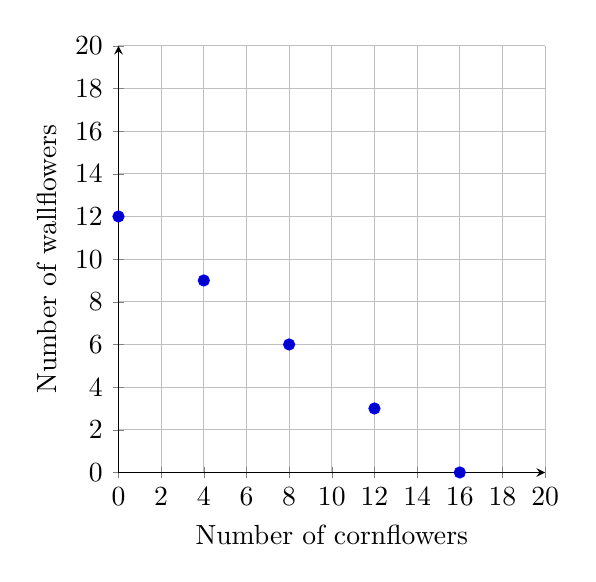
\begin{tikzpicture}
  \begin{axis}[
    width=7cm, height=7cm,
    grid=major,
    xmin=0, xmax=20,
    ymin=0, ymax=20,
    xlabel=Number of cornflowers,
    ylabel=Number of wallflowers,
    xtick={0,2,...,20},
    ytick={0,2,...,20},
    enlargelimits=false,
    axis lines=left,
    every axis plot/.append style={only marks, mark=*}
  ]
  \addplot coordinates {
    (0,12)
    (4,9)
    (8,6)
    (12,3)
    (16,0)
  };
  \end{axis}
\end{tikzpicture}
\end{center}

\vspace{2em}
\noindent\markforreview

\vspace{1em}

The graph of \( 7x + 2y = -31 \) in the \( xy \)-plane has an \( x \)-intercept at \( (a, 0) \) and a \( y \)-intercept at \( (0, b) \), where \( a \) and \( b \) are constants. What is the value of \( \frac{b}{a} \)?

\vspace{0.75em}

\choicebox{A}{$-\frac{7}{2}$}
\choicebox{B}{$-\frac{2}{7}$}
\choicebox{C}{$\frac{2}{7}$}
\choicebox{D}{$\frac{7}{2}$}

\newpage
\noindent\markforreview

\vspace{1em}

Line $\ell$ in the $xy$-plane is perpendicular to the line with equation $x = 2$. What is the slope of line $\ell$?

\vspace{0.75em}

\choicebox{A}{$0$}
\choicebox{B}{$\dfrac{1}{2}$}
\choicebox{C}{$-2$}
\choicebox{D}{The slope of line $\ell$ is undefined.}


\vspace{5em}
\noindent\markforreview

\vspace{1em}

The graph of \( 9x - 10y = 19 \) is translated down 4 units in the xy-plane. What is the x-coordinate of the x-intercept of the resulting graph?


\vspace{5em}
\newpage
\noindent\markforreview

\vspace{1em}

The table above shows the coordinates of three points on a line in the xy-plane, where \( k \) and \( n \) are constants. If the slope of the line is 2, what is the value of \( k + n \)?

\[
\begin{array}{c|c}
x & y \\
\hline
3 & 7 \\
k & 11 \\
12 & n \\
\end{array}
\]

\vspace{5em}

\noindent\markforreview

\vspace{1em}

In the given pair of equations, \( a \) and \( b \) are constants. The graph of this pair of equations in the xy-plane is a pair of perpendicular lines. Which of the following pairs of equations also represents a pair of perpendicular lines?

\[
\begin{aligned}
5x + 7y = 1 \\
ax + by = 1 \\
\end{aligned}
\]

\vspace{0.75em}

\choicebox{A}{\(10x + 7y = 1 \quad\) and  \(2ax + 5by = 1\)}
\choicebox{B}{\(10x + 7y = 1 \quad\) and  \(ax + 2by = 1\)}
\choicebox{C}{\(10x + 7y = 1 \quad\) and  \(2ax + by = 1\)}
\choicebox{D}{\(5x - 7y = 1 \quad\) and  \(ax + by = 1\)}

\newpage

\noindent\markforreview

\vspace{1em}

At a school fair, students can win colored tokens that are worth a different number of points depending on the color. One student won \( G \) green tokens and \( R \) red tokens worth a total of 380 points. The given equation represents this situation. How many more points is a red token worth than a green token?

\[
5G + 45R = 380
\]

\vspace{2em}
\noindent\markforreview

\vspace{1em}

To earn money for college, Avery works two part-time jobs: A and B. She earns \$10 per hour working at job A and \$20 per hour working at job B. In one week, Avery earned a total of \( s \) dollars for working at the two part-time jobs. The graph below represents all possible combinations of numbers of hours Avery could have worked at the two jobs to earn \( s \) dollars. What is the value of \( s \)?

\begin{center}
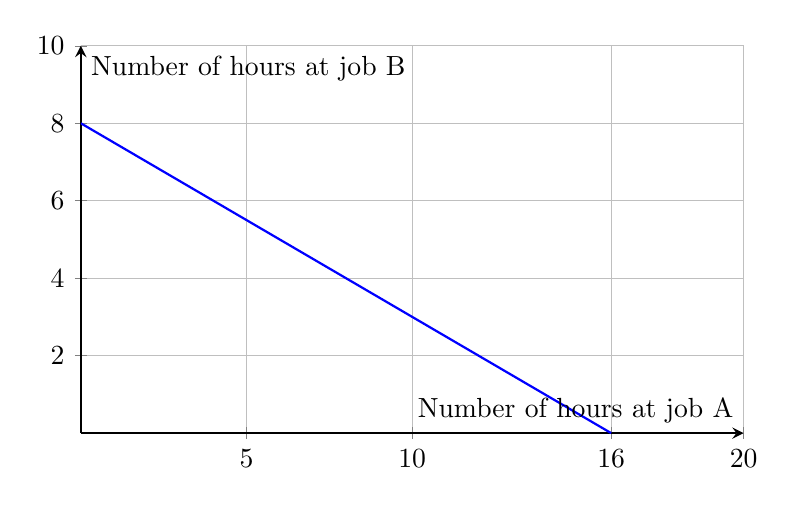
\begin{tikzpicture}
  \begin{axis}[
    width=10cm,
    height=6.5cm,
    xmin=0, xmax=20,
    ymin=0, ymax=10,
    axis lines=middle,
    xlabel={Number of hours at job A},
    ylabel={Number of hours at job B},
    xtick={0,5,10,16, 20},
    ytick={0,2,4,6,8,10},
    grid=major,
    thick
  ]
    % Plot the line y = 10 - 0.5x
    \addplot[
      domain=0:20,
      samples=100,
      thick,
      color=blue
    ] coordinates{(0,8)
    (16,0)};
  \end{axis}
\end{tikzpicture}
\end{center}




\choicebox{A}{128}
\choicebox{B}{160}
\choicebox{C}{200}
\choicebox{D}{320}

\newpage
\noindent\markforreview

\vspace{1em}

The line with the equation \( \frac{4}{5}x + \frac{1}{3}y = 1 \) is graphed in the \( xy \)-plane.

\vspace{2mm}
What is the x-coordinate of the x-intercept of the line?


\vspace{2em}

\noindent\markforreview

\vspace{1em}

\begin{center}
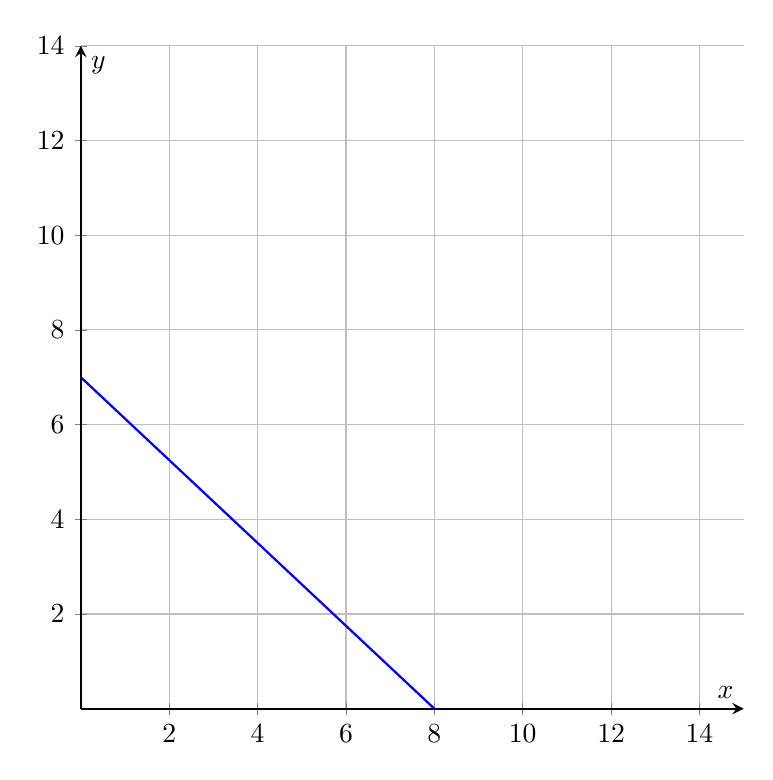
\begin{tikzpicture}
  \begin{axis}[
    width=10cm,
    height=10cm,
    xmin=0, xmax=15,
    ymin=0, ymax=14,
    axis lines=middle,
    xlabel={$x$},
    ylabel={$y$},
    xtick={0,2,...,14},
    ytick={0,2,...,14},
    grid=major,
    thick
  ]
    \addplot[domain=0:10, samples=2, thick, color=blue] coordinates{(0,7)
    (8,0)}; % Equation: y = -x + 10
  \end{axis}
\end{tikzpicture}
\end{center}

The point with coordinates $(d, 4)$ lies on the line shown. What is the value of $d$?

\vspace{0.75em}

\choicebox{A}{$\frac{7}{2}$}
\choicebox{B}{$\frac{26}{7}$}
\choicebox{C}{$\frac{24}{7}$}
\choicebox{D}{$\frac{27}{8}$}

\vspace{2em}

\noindent\markforreview

\vspace{1em}

In the $xy$-plane, line $k$ is defined by $x + y = 0$. Line $j$ is perpendicular to line $k$, and the $y$-intercept of line $j$ is $(0,3)$. Which of the following is an equation of line $j$?

\vspace{0.75em}

\choicebox{A}{$x + y = 3$}
\choicebox{B}{$x + y = -3$}
\choicebox{C}{$x - y = 3$}
\choicebox{D}{$x - y = -3$}


\vspace{2em}

\noindent\markforreview

\vspace{1em}

How many liters of a 25\% saline solution must be added to 3 liters of a 10\% saline solution to obtain a 15\% saline solution?


\newpage
